\chapter{Garfield++}


\section{Introducción}

\textbf{Garfield++} es una herramienta basada en la programación orientada a objetos que permite simulaciones detalladas de detectores de partículas basadas en ionización de gases o semiconductores. Para calcular los campos eléctricos, se ofrecen ls siguientes técnicas: 

\begin{itemize}
    \item Soluciones para hilos/cables finos para detectores basados en hilos y planos. 
    \item Interfaces\footnote{Conexión funcional entre dos sistemas, programas, dispositivos o componentes de cualquier tipo, que proporciona una comunicación de distintos niveles, permitiendo el intercambio de información.} para elementos finitos, que pueden calcular campos aproximados en configuraciones 2 y 3 dimensionales con materiales dieléctricos y conductores. 
\end{itemize}
Para calcular las propiedades de tranpsorte de las partículas en mezclas de gases, usamos la interfaz de Magboltz. La ionización producida por partículas cargadas relativistas se estudia a través del programa Heed. Para la simulación de ionización producida por iones a baja energía, los resultados puede ser estudiado por el paquete SRIM. El programa Degrade simula la ionizacion producida por electrones. 



\begin{Ejemplo}{\textbf{Tubo de deriva}}

En est ejemplo vamos a considerar un tubo de deriva con un diámetro de 15 mm y un diámetro del hilo (cable) de 50 $\mu m$, similar a los tubos de derivas de muones del ATLAS (también con un diámetro pequeño) llamados sMDTs. Primero importamos los módulos: \\

\begin{lstlisting}[language=C++,style=c++]
#include "Garfield/MediumMagboltz.hh"
#include "Garfield/ViewMedium.hh"
\end{lstlisting}

\vspace*{1em}


Lo primero que tenemos que hacer es preparar la \textbf{tabla de gases}, es decir, la tabla que contiene los parámetros de transporte (velocidad de deriva, coeficientes de difusión, coeficiente de Townsend, coeficiente de captura) como funciones del campo eléctrico $\Encal$ (y en general, del campo magnético $\Bn$ y el ángulo entre $\Encal$ y $\Bn$) para un gas a una temperatura y presión determinadas. En este ejemplo usaremos un gaz mezcla, a 3 atm y temperatura ambiente: \\

\begin{lstlisting}[language=C++,style=c++]
MediumMagboltz gas("ar", 93., "co2", 7);
// Set temperature [K] and preasure [Torr]
gas.SetPressure(3*760.);
gas.SetTemperature(293.15);
\end{lstlisting}

\vspace*{1em}

También debemos especificar el número de puntos de la malla campo eléctrico que vamos a usar en la tabla y el rango que va a ser cubierto. Usamos 20 puntos entre 100 V/cm a 100 kV/cm con un espaciado logaritmico:   \\

\begin{lstlisting}[language=C++,style=c++]
gas.SetFieldGrid(100.,100.e3,20,true);
\end{lstlisting}

\vspace*{1em}
    
Ahora ejecutamos Magboltz para generar una tabla del gas para esta malla de campo eléctrico. Como un parámetro de entrada tenemos que especificar \textit{el número de colisiones} (en múltiplos de $10^7$) sobre el electrón cuya traza dibuja Magboltz: \\

\begin{lstlisting}[language=C++,style=c++]
const int ncolll=10;
\end{lstlisting} 

Aunque tarde un rato, una vez este acabado podemos guardar los parámetros:  \\

\begin{lstlisting}[language=C++,style=c++]
gas.WriteGasFile("ar_93_co2_7.gas");
\end{lstlisting} 

\vspace*{1em}

para luego poder importarlos cuando queramos, y no tener la necesidad de correr el programa cada vez que los queramos: \\


\begin{lstlisting}[language=C++,style=c++]
gas.LoadGasFile("ar_93_co2_7.gas");
\end{lstlisting} 

\vspace*{1em}

Una buena idea podría ser, para asegurarse que el cálculo es correcto, graficar la velocidad de deriva en función del campo eléctrico: \\

\begin{lstlisting}[language=C++,style=c++]
ViewMedium view;
view.SetMedium(&gas);

// Dibujamos: 
TCanvas* c1 = new TCanvas("c1", "Propiedades del gas", 800, 600);
view.PlotElectronVelocity();
c1->SaveAs("drift_velocity.pdf");
\end{lstlisting} 

\begin{center}
    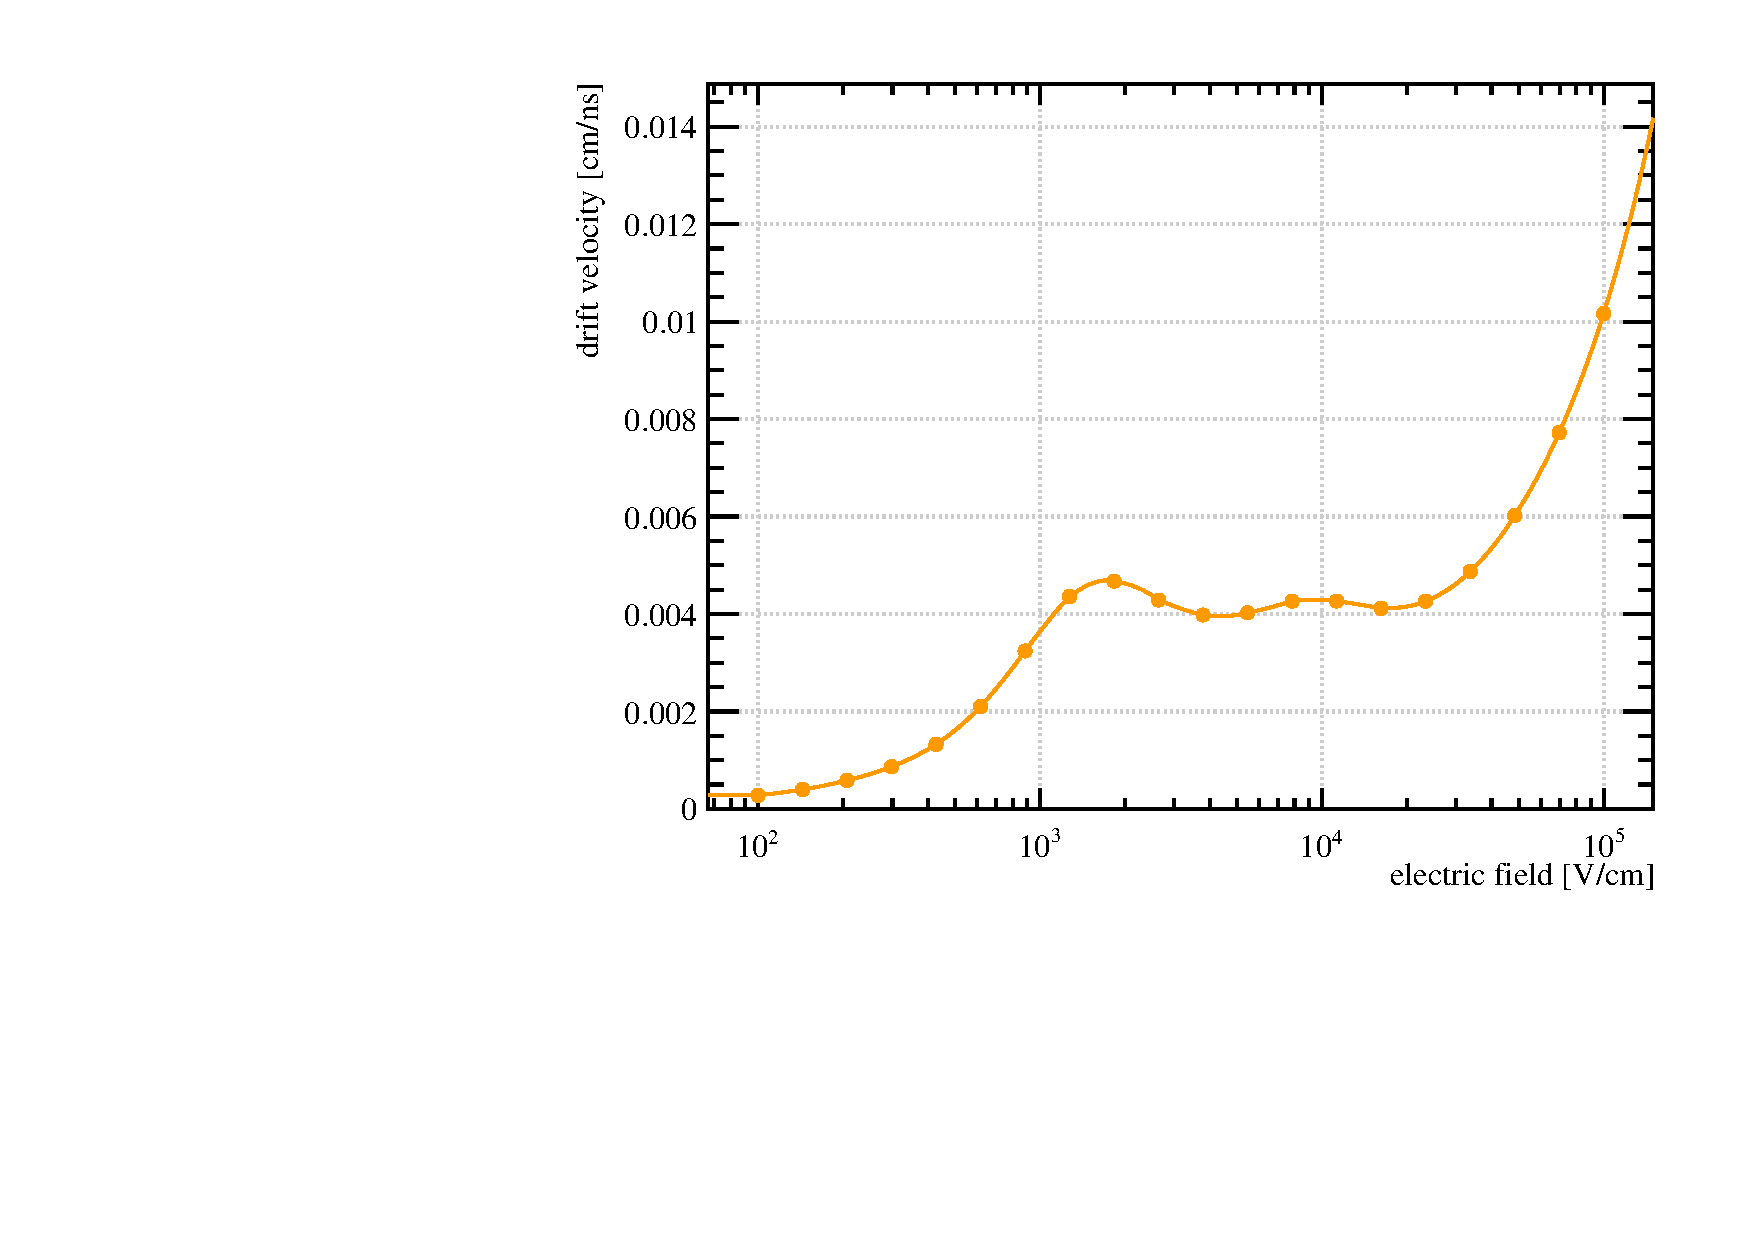
\includegraphics[width=0.6\linewidth]{Chapters/EjemploGarfield/TuboDeriva/build/drift_velocity.pdf}
\end{center}

Ahora podemos calcular el  \textbf{campo eléctrico} que se hace a través de \texttt{ComponentAnalyticField}, que básicamente maneja la disposición de cables, planos y tubos: \\

\begin{lstlisting}[language=C++,style=c++]
ComponentAnalyticField cmp;
\end{lstlisting} 

\vspace*{1em}

Tenemos que introducir el medio que hemos definido en la región activa: \\

\begin{lstlisting}[language=C++,style=c++]
cmp.SetMedium(&gas);
\end{lstlisting} 

\vspace*{1em}

Lo siguiente que tenemos que hacer es añadir los elementos que definen el campo eléctrico, i.e. el cable (denominado ``s'') y el tubo: \\


\begin{lstlisting}[language=C++,style=c++]
// Radio del cable [cm]
const double rWire = 25.e-4;

// Radio del tubo externo [cm]
const double rTube = 0.71;

// Voltajes 
const double vWire = 2730.;
const double vTube =    0.;

// Añadimos el cable en el centro de la disposición 
cmp.Addwire(0,0,2 * rWire, vWire, "s");

// Añadimos el tubo
cmp.AddTube(rTube, vTube, 0);
\end{lstlisting} 
\vspace*{1em}

Finalmente, creamos un \texttt{Sensor}, que es un objeto que actúa como interfaz en la clase transporte  discutido más abajo: \\


\begin{lstlisting}[language=C++,style=c++]
// Calculamos el campo eléctrico usando el objeto Componente cmp.
Sensor sensor(&cmp);
// Hacemos una petición para que calcule la señal del electrodo llamado s
//     usando el campo dado por el objeto Componente cmp.
sensor.AddElectrode(&cmp,"s");
\end{lstlisting} 
\vspace*{1em}

Ahora necesitadmos definir el intervalo temporal en el que la señal es guardada y la granularidad (ancho del bin). Podemos usar 1000 bins con un ancho de 0.5 ns \\

\begin{lstlisting}[language=C++,style=c++]
const double tstep = 0.5;
const double tmin = -0.5 * tstep;
const unsigned int nbins = 1000;
sensor.SetTimeWindow(tmin,tstep,nbins);
\end{lstlisting} 
\vspace*{1em}

Ahora lo que nos queda es \textbf{simular la ionización producida} por la partícula en el tubo de carga usando Heed, de un muón, con por ejemplo, 170 GeV. \textit{Track} significa camino o trayectoria en ingles. \\

\begin{lstlisting}[language=C++,style=c++]
TrackHeed track(&sensor);
track.SetParticle("muon");
track.SetEnergy(170.e9);
\end{lstlisting} 
\vspace*{1em}

Las curvas (lineas) de deriva de los electrones se crean usando el método de integración Runge-Kutta:fehlberg (RKF), implementada en la clase \texttt{DriftLineRKF}. Este método usa las tablas previamente computadas de parámetros de transporte para calcular las líneas de deriva y su multiplicación: \\


\begin{lstlisting}[language=C++,style=c++]
DriftLineRKF drift(&sensor);
\end{lstlisting} 
\vspace*{1em}

Consideremos ahora que la pista pasa a una distancia de 3 mm del centro del hilo. Después de simular el paso de la partícula cargada, nos tenemos que fijar en los ``clusters'' (agrupaciones de partículas cargadas producidas por la partícula primaria) y su movimiento en el dispositivo. Así pues, calculamos las líneas de deriva para cada electrón producido en el cluster: 

\begin{lstlisting}[language=C++,style=c++]
const double rTrack = 0.3;
const double x0=rTrack;
const double y0 = -sqrt(rTube * rTube - rTrack * rTrack)
track.NewTrack(x0,y0,0,0,0,1,0);
// Hacemos un bucle sobre los clusters producidos por el camino (track)
for (const auto& cluster: track.GetClusters()) {
    // Bucle alrededor de los electrones del cluster
    for (const auto& electron: cluster.electrons) {
        drift.DriftElectron(electron.x,electron.y,electron.z,electron.t)
    }
}
\end{lstlisting} 
\vspace*{1em}

Como una comprobación de la simulación podemos visualizar las líneas de deriva. Antes de simular el recorrido de la partícula cargada y las curvas de deriva de los electrones, tenemso que decirle a \texttt{TrackHeed} y \texttt{DriftLineRKF} que pase las coordenadas de los clusters y los puntos de las líenas de deriva al objeto \texttt{ViewDrift}, que se encarga de graficarlas:  \\

\begin{lstlisting}[language=C++,style=c++]
// Creamos un canvas
cD = new TCanvas ("cD"," ", 600, 600);
ViewDrift driftView;
drift.EnablePlotting(&driftView);
track.EnablePlotting(&driftView);
cellView.SetCanvas(cD);
cellView.Plot2d();
constexpr bool twod=true;
constexpr bool drawaxis = false;
driftView.Plot(twod,drawaxis);
cD->SaveAs("drift_view.pdf");
delete cD;
\end{lstlisting} 
\vspace*{1em}
Podemos graficar la señal inducida en el hilo/cable por la deriva de los electrones simulados:  \\

\begin{lstlisting}[language=C++,style=c++]
TCanvas* cS = new TCanvas("cS","",600,600);
sensor.PlotSignal("s",cS);
\end{lstlisting} 
\vspace*{1em}

\begin{center}
    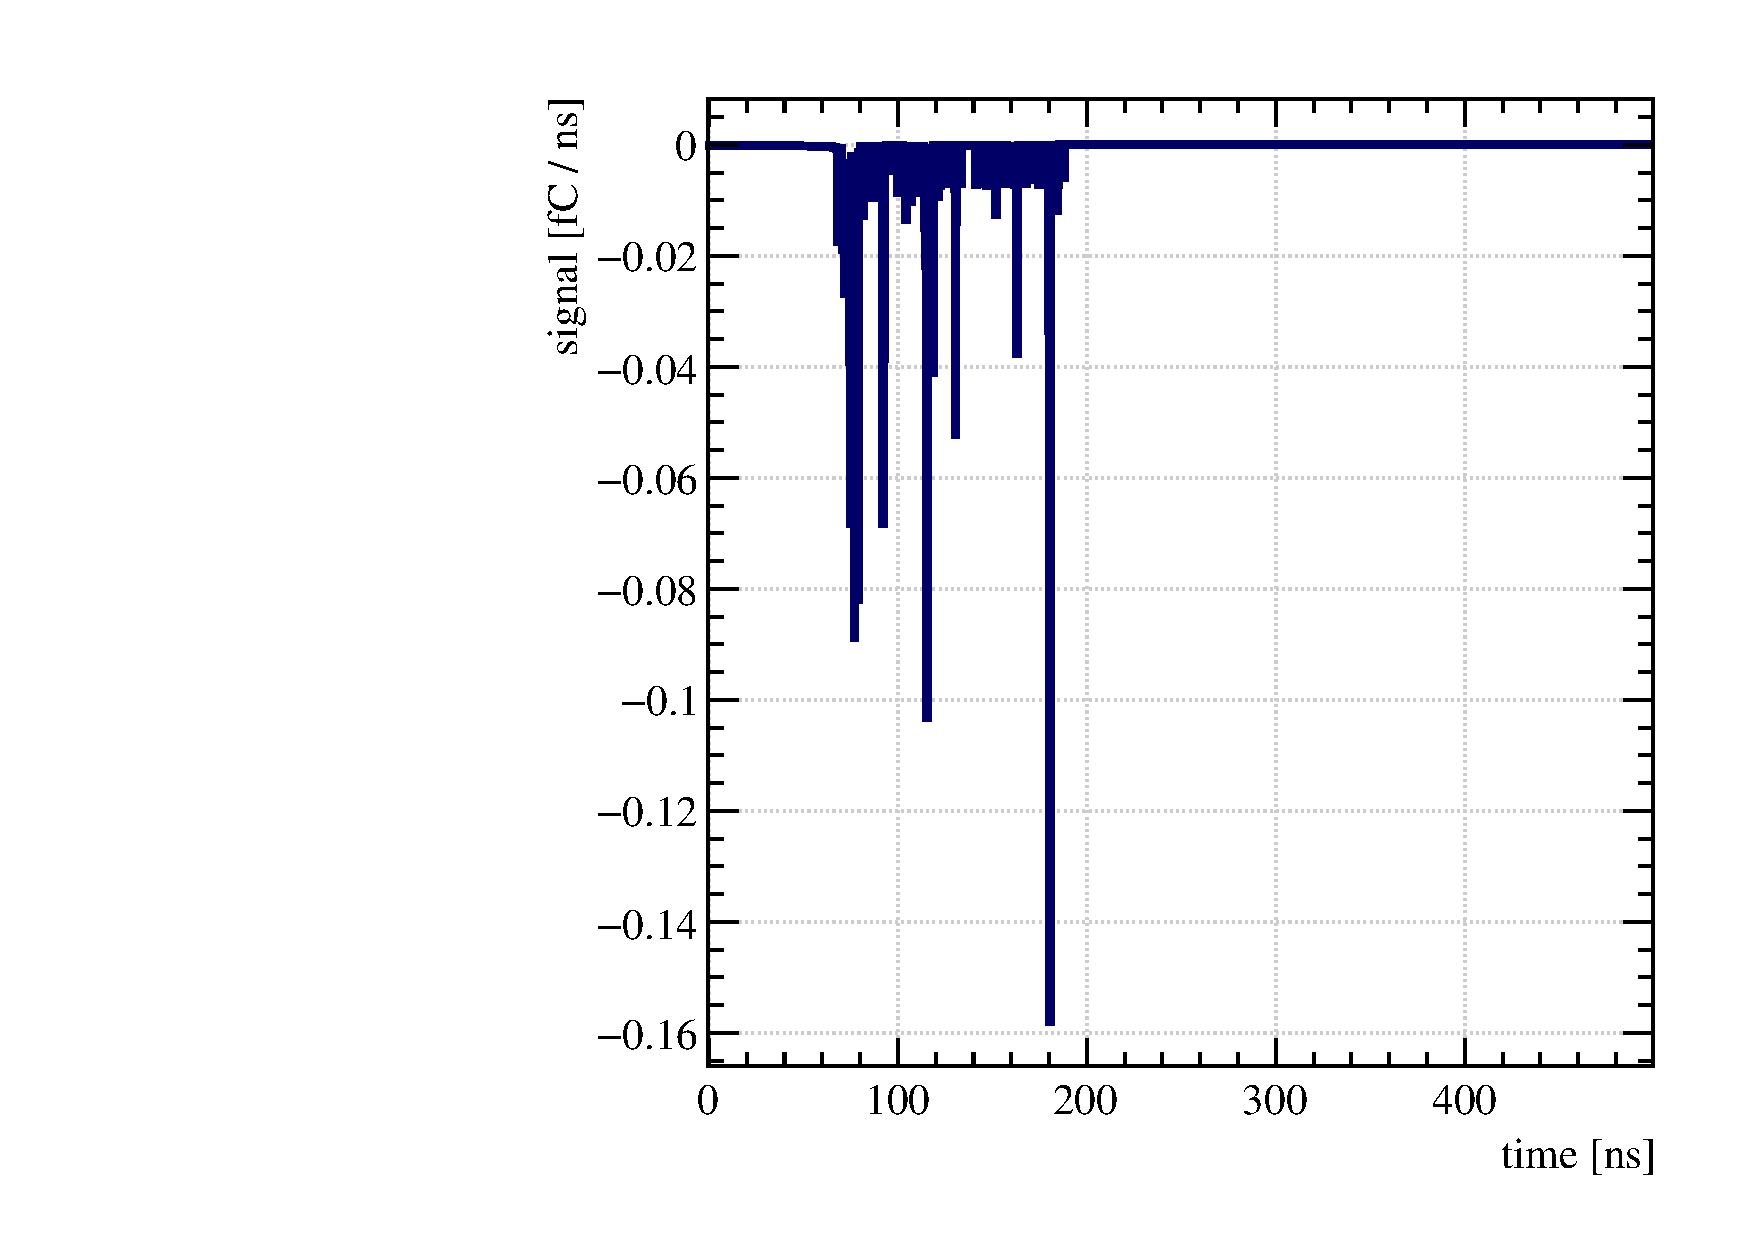
\includegraphics[width=0.6\linewidth]{Chapters/EjemploGarfield/TuboDeriva/build/signal.pdf}
\end{center}

Si quisieramos considerar la contribución de los iones producidos en la avalancha necesitamos importar tablas de mobilidades de iones: \\


\begin{lstlisting}[language=C++,style=c++]
gas.LoadIonMobility("LoadIonMobility_Ar+_Ar.txt")
\end{lstlisting} 
\vspace*{1em}

que, por defecto, \texttt{DriftLineRKF} las incluirá en la simulación. 






\end{Ejemplo}

\section{Media}

\section{Components}

\section{Tracks}

El propósito de las clases \texttt{Track}\footnote{\textit{Track} se puede traducir como camino, trayectoria, pista, estela, senda...} son simular los procesos de ionización producidos por partículas cargadas atravesando el detector. Básicamente lo primero que hay que hacer es definir la partícula: \\

\begin{lstlisting}[language=C++,style=c++]
void SetParticle(std::string particle);
track.SetParticle(std::string particle);
\end{lstlisting}
\vspace*{0.7em}
como por ejemplo puede ser  \texttt{"muon"}. La cinemática de la partícula cargada puede definirse de diferntes formas:

\begin{itemize}
    \item Con la energía total en eV.
    \item Con la energía cinética en eV.
    \item Con el momento en eV/c.
    \item Con la velocidad $\beta$ adimensional, el factor de Lorenzt $\gamma$ o el producto $\beta\gamma$. 
\end{itemize}

\begin{lstlisting}[language=C++,style=c++]
// Métodos de establecimiento de variables físicas
void SetEnergy(const double e);
void SetKineticEnergy(const double ekin);
void SetMomentum(const double p);
void SetBeta(const double beta);
void SetGamma(const double gamma);
void SetBetaGamma(const double bg);
\end{lstlisting}
\vspace*{0.7em}
El track se inicializa mediante:   \\ 
\begin{lstlisting}[language=C++,style=c++]
void NewTrack(const double x0, cons double y0, const double z0, const double t0, const double dx0, const double dy0, const double dz0)
\end{lstlisting}
\vspace*{0.7em}
Los marcadores \texttt{x0, y0} y \texttt{z0} marcan la \textit{posición inicial} en cm, \texttt{t0} el \textit{instante inicial} y \texttt{dx0, dy0, dz0} el \textit{vector inicial}. El punto inicial del recorrido tiene que estra dentro del medio. Si la dirección del vector es nula, un vector aleatorio isótropo será generado. Dependiendo del tipo de clase \texttt{Track} que se use, mas restricciones podrán ser impuestas. 

Tras la inicialización, los ``cluster'' se producen a lo largo del recorrido, que se pueden obtener con: \\

\begin{lstlisting}[language=C++,style=c++]
const std::vector<Cluster>& GetClusters();
\end{lstlisting}
\vspace*{0.7em}
Cuando hablamos de ``cluster'' nos refereimos a la energía cedida en una única interacción ionizante de la partícula primaria cargadam y los electrones  secundarios producidos en este proceso. La implementación concreto de los objetos Cluster dependen de la clase \texttt{Track} de la que estemos hablando. 

\subsection{Heed}

El programa Heed es una implementación del modelo de la ionización por foto-abosrción (también llamado modelo PAI, \textit{photo-absorption model}, PAI), escrito por I. Smirnov. La interfaz Heed está disponible a través de \texttt{TrackHeed}.

Los objetos \texttt{Cluster} se obtienen a través de \texttt{TrackHeed::GetClusters} contiene la posición y tiempo de la colisión ionizante, la energía transferida y el vector de objetos \texttt{Electron} correspondientes a los electrones conductores/libres\footnote{son simplemente los electrones libres en el gas.} asociados al cluster. 

\subsubsection{Transporte de electrones Delta}

Heed simula el tiempo de degradación de los electrones $\delta$ y la producción de electrones secundarios (electrones conductores/libres) usando un modelo fenomenolóicos. \texttt{TrackHeed} recupera los parámetros de entrada necesarios (por ejemplo el el factor de Fano o el valor $W$) del objeto \texttt{Medium}. Si los parámetros son cero, usa los valores por defecto (por ej. $F=0.19$).


Si los electrones delta son desactivados, el número de electrones devuelto por el \texttt{GetCluster} es el número de electrones primarios (electrones producidos por la ionización primaria), i.e. foto-electrones y electrones Auger. Las enerǵias cinéticas y posiciones de los electrones son acesibles vía \texttt{GetElectron}. Si el tranpsorte de electrones $\delta$ está activado (por defecto está activado), la función \texttt{GetElectron} devuelve la localización de los electrones de conducción calculados por el factor interno $\delta$ del algoritmo de Heed. Dado que este método no devuelve la energía cinética y dirección de los electrones secundarios, los parámetros de \texttt{GetElectron} no son significativos en este caso.

\subsubsection{Transporte de fotones}

Heed también puede simular la fotoabsorción de rayos-x. 

\subsubsection{Campos magnéticos}

Si el \texttt{sensor} tiene un campo magnético nulo, \texttt{TrackHeed} lo tnedrá en cuenta para calcular la trayectoria de la partícula cargada.

\subsection{SRIM}

SRIM (\textit{Stopping and Range of Ions in Matter}) es un programa que permite simular la perdida de energía iónica por la materia en la materia. Esto produce tablas de frenados energéticos, rangos y parámetros de \textit{stragglings}\footnote{Recordemos que el straggling es el fenómeno que recoge las fluctuaciones estadísticas asociadas a las pérdidas energéticas.} que pueden ser importados en Garfield a través de la clase \texttt{TrackSrim}. La función: \\

\begin{lstlisting}[language=C++,style=c++]
bool ReadFile(const std::string& file)
\end{lstlisting}
\vspace*{0.6em}
devuelve \texttt{true} si es leido correectamente. Los archivos SRIM contiene la siguiente información: 

\begin{itemize}
    \item Una lista de energías cinéticas en las que se han calculado pérdidas y rezagos;
    \item Energía promedio perdida por unidad de longitud vía proceos electromagnéticos, para cada enerǵia. 
    \item Energía promedio perdida por unidad de longitud vía proceos nucleares, para cada enerǵia. 
    \item Proyección de l4!a media recorrida, por energía.
    \item Straggling longitudinal y transversal para cada energía. 
\end{itemize}
Se pueden visualizar usando las funciones: \\

\begin{lstlisting}[language=C++,style=c++]
void PlotEnergyLoss();
void PlotRange();
void PlotStraggling(); 
\end{lstlisting}
\vspace*{0.6em}

Además de estas tablas, el archivo también contiene la masa y carga del proyectil y la densidad del medio. Estas propiedades son también emportantes y guardadas por \texttt{TrackSrim} cuando leemos el archivo. Al contrario del caso Heed, el tipo de partícula no es especificada por el usuario, aunqeu si tenga que especificar la energía cinética del proyectil.

El \texttt{TrackSrim} genera reocrridos individuales que estadísiticamente representan las cantidades promedio calculadas por SRIM. Una vez se pasa la energía, \texttt{TrackSrim}, interativamente

\begin{itemize}
    \item Calcula (interpolando las tablas) la energía electromagnética y nuclear perdida por unidad de distancia para dicha energía.
    \item Calcula la longitud del paso/intervalo (\textit{step}) en el cual la energía producirá una cantidad de electrones promedio. .
    \item Actualiza la trayectoria basada en el la dispersión longitudinal y transerval para la energía de la partícula. 
    \item Calcula una pérdida energía electromagnética aleatoria sobre el intervalo y actualiza la energía cinética.
\end{itemize}
repitiendo el proceso hasta que la partícula ya no tiene maś energía o deja de estar en la geometría (dispositivo). Se pueden elegir varios modelos por los cuales se aleatoriza la péridda de energía en cada paso

\begin{lstlisting}[language=C++,style=c++]
void SetModel(const imt m) 
\end{lstlisting}
\vspace*{0.6em}
En función de $m$ tendremos un modelo u otro. Los modelos disponibles son: 

\begin{table}[h!]
\centering
\begin{tabular}{ll}
\toprule
\textbf{Modelo} & \textbf{Descripción} \\
\midrule
0 & Sin fluctuaciones \\
1 & Distribución de Landau no truncada \\
2 & Distribución de Vavilov (siempre que los parámetros cinemáticos estén dentro del \\ & rango de aplicabilidad de lo contrario, las fluctuaciones se desactivan) \\
3 & Distribución gaussiana \\
4 & Combinación de los modelos de Landau, Vavilov y Gauss, cada \\
  &  uno aplicado en su supuesto dominio de aplicabilidad \\
\bottomrule
\end{tabular}
\end{table}

Para samplear las pérdidas energéticas, \texttt{TrackSrim} necesita la densidad delectrónica del material, que por defecto se recupera del objeto \texttt{Medium} (y escalada con la densidad de masa del archivo SRIM). Tambień se puuede usar un número $Z$ efectivo y el número másico $A$ usando

\begin{lstlisting}[language=C++,style=c++]
{TrackSrim::SetAtomicMassNumbers}.
\end{lstlisting}
\vspace*{0.6em}


Para calcular el número de electrones generados para una energía depositada, \texttt{TrackSrim} necestia la función de trabajo $W$ en eV y el factor de Fano del material, qeu se pedirán al objeto \texttt{Medium}, aunque puede ser dado a mano. El objeto \texttt{Cluster} devuelto por \texttt{TrackSrim::GetClusters} contiene la localización y tiempo inicial del cluster, la energía gastada para producir el cluster, la energía del ion cuando el cluster fue creado y el número de elctrones por cluster. 

\subsection{TRIM}

TRIM (\textit{TRansport of Ions in Matter}) es una simulación montecarlo del mismo conjunto de programas que SRIM, que simula la trayectoria individual de un ión en en el medio y su proceso de pérdida de energía (cascadas de retroceso, daños por desplazamiento...). TRIM produce típicamente un número determinado de archivos de salida, entre los cuales EXYZ.txt que contiene la lista de posición y pérdidas de energía electrónicas para cada ion simulado en pasos regularess.

\subsection{Degrade}

La clase \texttt{TrackDegrade} simula las ionizaciones por electrones primarios en el gas y la subsecuente degradación en electrones $\delta$ (electrón que puede recorrer cierta distancia antes de perder energía y provocar ionización secundaria a lo largo de su camino.), electrones Auger (surgen de la reorganización interna del átomo cuando la energía de una transición electrónica se transfiere a otro electrón que es expulsado) y fotoelectrones (fotoelectrones se originan por la absorción de un fotón, mientras que los electrones Auger), usando una interfaz al programa Degrade, desarrollado por S. Biagi. Degrade tiene muchos puntos en común con Magboltz, en particular la base de datos de secciones eficaces de electrón-átomo/molécula. 

Mientras el programa Degrade puede ser usado para la simulación de rayos X, los decaimientos $\beta$ y doble $\beta$, estas características aún no han sido implementadas, al igual que no contiene las interacccioens en presencia de campo eléctrico y magnético. 


Los objetos \texttt{Cluster} devuletos por \texttt{TrackDegrade::GetClusters} contienen la posición y tiempo de las colisiones ionizantes (\texttt{x,y,z,t}) y un \texttt{vector} de objetos \texttt{Electron} correspondientes a electrones termializados asociados al cluster. Además, contiene un vector de electrones delta y Auger. \\


\begin{lstlisting}[language=C++,style=c++]
TrackDegrade track;          // Se crea un objeto de tipo TrackDegrade 

// Variables iniciales de posición y tiempo:
double x0 = 0., y0 = 0., z0 = 0., t0 = 0.;

// Dirección inicial del movimiento:
double dx0 = 1., dy0 = 0., dz0 = 0.;

// Se genera una nueva trayectoria con las condiciones iniciales anteriores:
track.NewTrack(x0, y0, z0, t0, dx0, dy0, dz0);

// Bucle sobre los "clusters" (agrupaciones de ionización o excitación) a lo largo de la trayectoria.
for (const auto& cluster : track.GetClusters()) {

    // Bucle sobre los electrones termalizados dentro del cluster.
    for (const auto& electron : cluster.electrons) {

        // Se obtienen las coordenadas y la energía cinética del electrón.
        double xe = electron.x;
        double ye = electron.y;
        double ze = electron.z;
        double te = electron.t;
        double ee = electron.energy;
    }
}
\end{lstlisting}
\vspace*{0.6em}
Por defecto, los electrones están \textit{trackeados} hasta que su energía cinética cae hasta 2eV. Esto peude ser modificado.  Si la función \\

\begin{lstlisting}[language=C++,style=c++]
void StoreExcitations(const bool on=true, const double ethr);
\end{lstlisting}
\vspace*{0.6em}
se llama antes de \texttt{NewTrack}, las excitaciones (con una energía de excitación superior a \texttt{ethr}) producidas por los electrones ionizantes primarios y secundarios se guardan en el objeto \texttt{Cluster}.

\section{Transporte de Carga}